\newpage
\section{NOTA TEÓRICA}

Antes de iniciar con el uso y manipulación del lenguaje de programación C para la creación de los algoritmos objetivo del presente laboratorio, es necesario tener a mano una serie de conceptos importantes, los cuales se explican a continuación: 

\subsection{Microcontrolador STM32F429}
Tal como se detalla en la hoja del fabricante \cite{ST}, el STM32F429 es un microcontrolador de 32 bits desarrollado por STMicroelectronics, perteneciente a la familia STM32, que se basa en el núcleo ARM Cortex-M4 que opera a una frecuencia de hasta 180 MHz.. Este microcontrolador es conocido por su alto rendimiento, amplia gama de periféricos y altas capacidades que lo hacen ideal para aplicaciones complejas en una variedad de campos, como la electrónica de consumo, la automatización industrial y las telecomunicaciones.

Incluye instrucciones específicas para el procesamiento digital de señales (DSP), que son particularmente útiles para aplicaciones que requieren cálculos matemáticos intensivos, una memoria flash con capacidad de 2 MB y una SRAM de 256Kb. Asimismo, cuenta con hasta 168 GPIO programables, 17 timers (6 timers generales de 16 bits y 4 timers generales de 32 bits). Posee un controlador TFT-LCD que permite la conexión directa a pantallas TFT, facilitando el desarrollo de interfaces gráficas. Soporte para interfaces de cámaras digitales, útil en aplicaciones de visión artificial. Incluye varios interfaces como USB OTG (On-The-Go), Ethernet, CAN (Controller Area Network), y varios puertos UART, SPI, I$^2$C, entre otros. Este microcontrolador dispone de 3 ADCs independientes de 12 bits, puede manejar hasta 24 canales, permitiendo la adquisición de señales de múltiples fuentes analógicas. 

En la Figura \ref{fig:ST_pins} puede observarse la distribución de pines del microcontrolador y sus respectivas funciones:  

\begin{figure}[H]
\centering
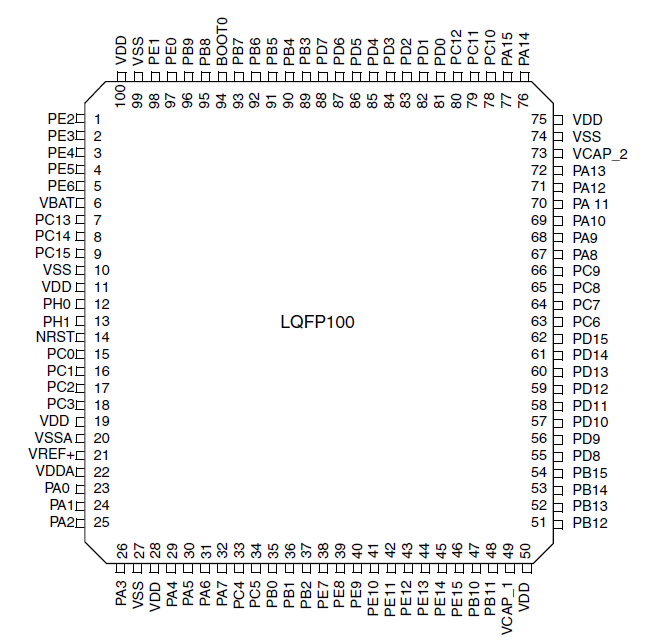
\includegraphics[scale=0.5]{./Figuras/Nota_teorica/PINES}
\caption{Diagrama de pines y sus respectivas funciones. (Fuente: Imagen tomada de \cite{ST})}
\label{fig:ST_pins}
\end{figure}

Para más información general del dispositivo, observar el Anexo \ref{an:01_GEN}. Por otro lado, en la Figura \ref{fig:DBLO} puede consultarse el diagrama de bloques del microcontrolador en el cual puede consultarse a alto nivel la conexión interna de este (no incluye el CPU):

\begin{figure}[H]
\centering
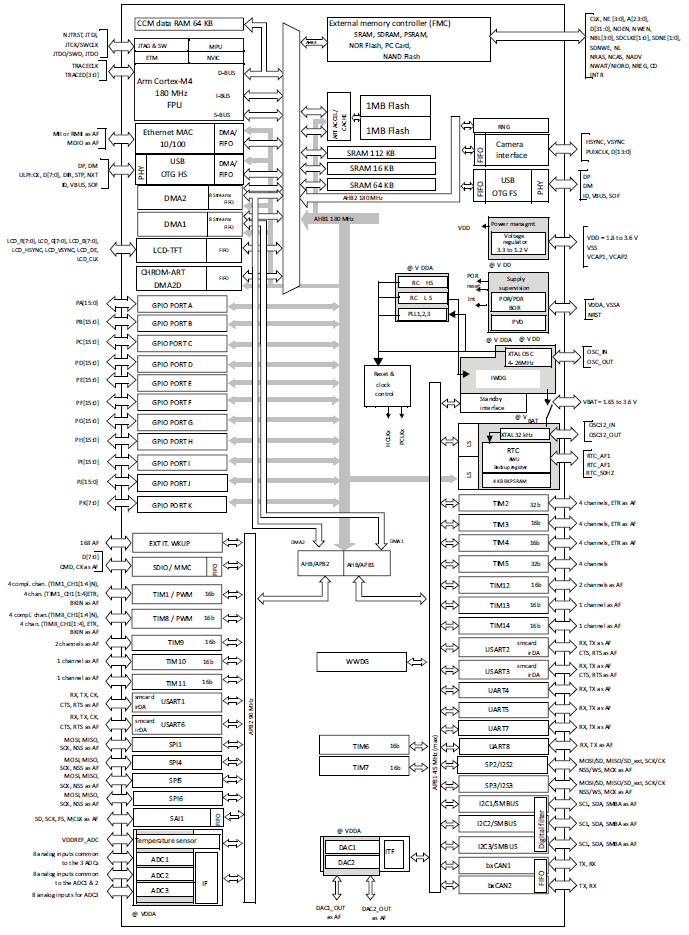
\includegraphics[width=160mm]{./Figuras/Nota_teorica/Bloques}
\caption{Diagrama de bloques del STM32F429. (Fuente: Imagen tomada de \cite{ST})}
\label{fig:DBLO}
\end{figure}



\subsubsection{Registros de importancia}
Según la hoja del fabricante \cite{ST}, el mapa de memoria del STM32F427xx y STM32F429xx está dividido en varias regiones, cada una asignada a diferentes tipos de periféricos y funcionalidades. A continuación, se muestran los rangos de direcciones de registros de importancia:

\begin{figure}[H]
\centering
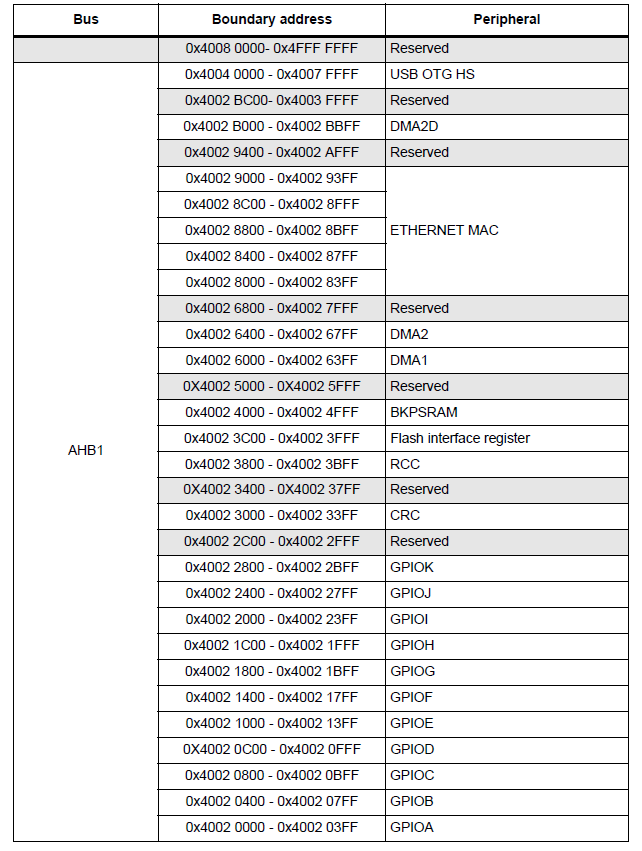
\includegraphics[scale=0.8]{./Figuras/Nota_teorica/REGS1}
\caption{Rangos direcciones de registros. (Fuente: Imagen tomada de \cite{ST})}
\label{fig:REGS1}
\end{figure}


\begin{figure}[H]
\centering
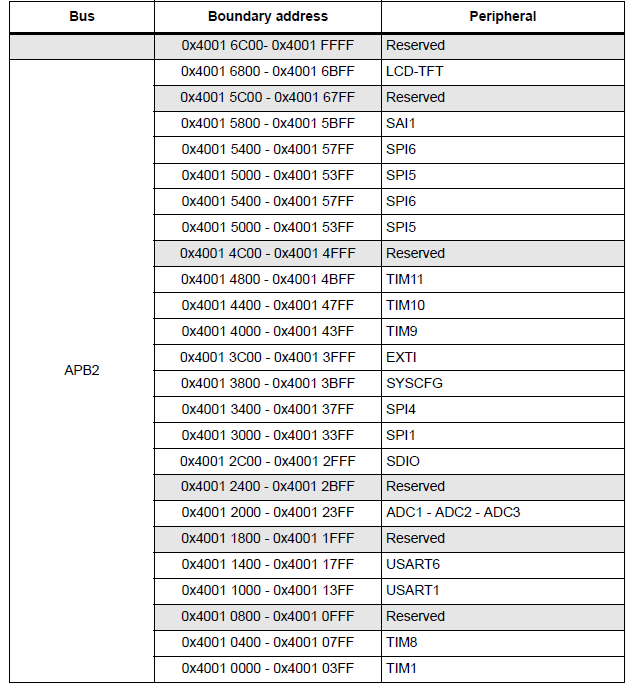
\includegraphics[scale=0.8]{./Figuras/Nota_teorica/REGS2}
\caption{Rangos direcciones de registros. (Fuente: Imagen tomada de \cite{ST})}
\label{fig:REGS2}
\end{figure}

\begin{figure}[H]
\centering
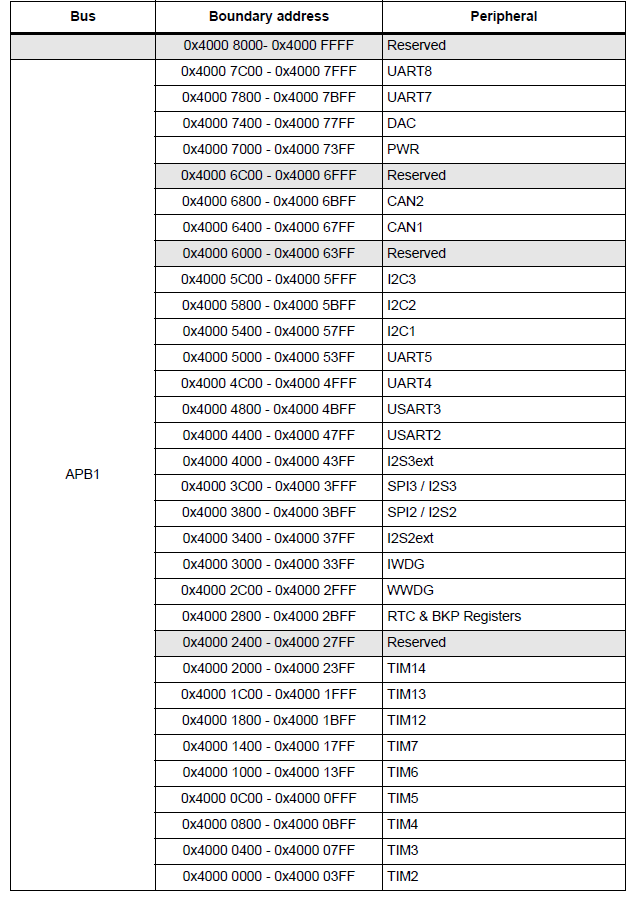
\includegraphics[scale=0.8]{./Figuras/Nota_teorica/REGS3}
\caption{Rangos direcciones de registros. (Fuente: Imagen tomada de \cite{ST})}
\label{fig:REGS3}
\end{figure}

Es importante mencionar que el caso de este microcontrolador, se puede utilizar ciertas librerías como LibOpenCM3 que proporcionan una capa de abstracción más alta sobre el hardware, lo que significa que facilita manipular los registros del microcontrolador.

\subsubsection{Características eléctricas}
A continuación se muestra las especificaciones eléctricas del STM32F429:

%%%%%%%%%%%%%%%%%%
\begin{figure}[H]
\centering
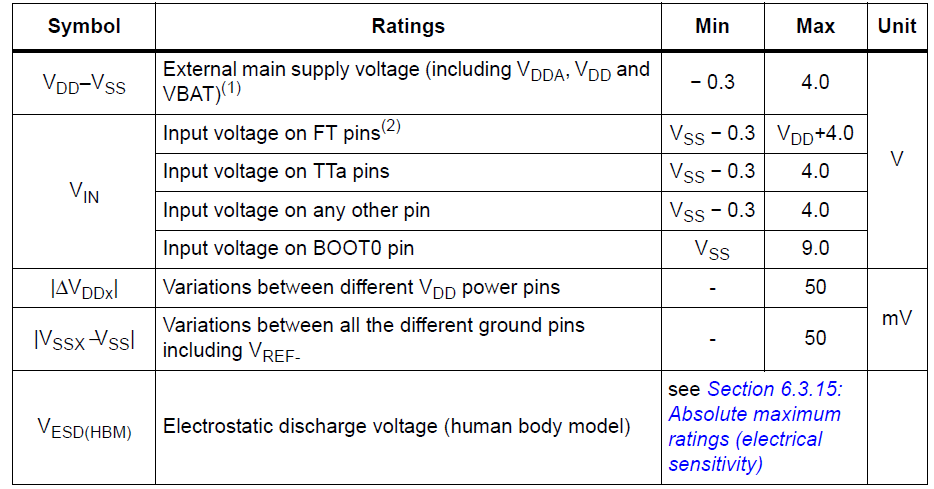
\includegraphics[scale=0.6]{./Figuras/Nota_teorica/ELEC1}
\caption{Características de tensión. (Fuente: Imagen tomada de \cite{ST})}
\label{fig:ELEC1}
\end{figure}

%%%%%%%%%%%%%%%%%%
\begin{figure}[H]
\centering
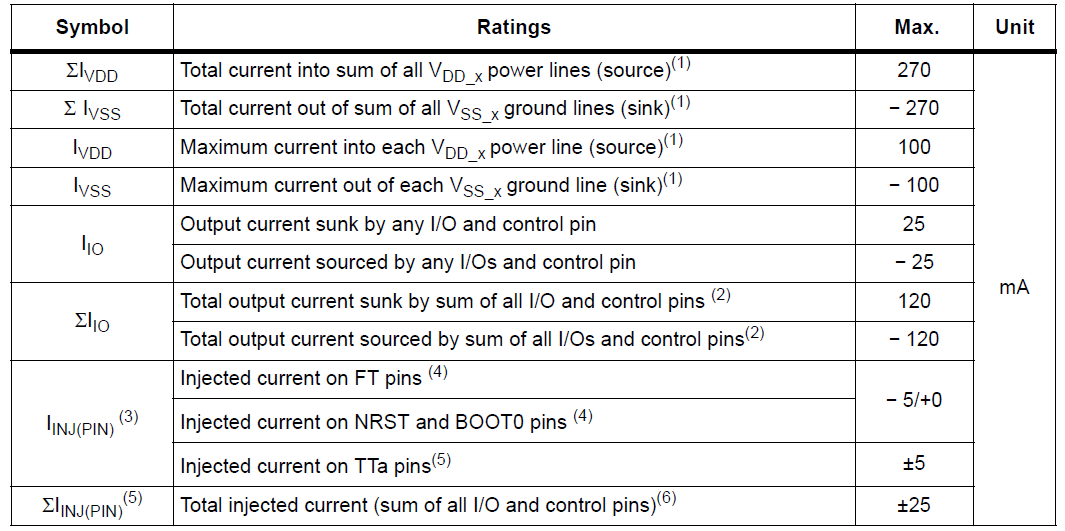
\includegraphics[scale=0.6]{./Figuras/Nota_teorica/ELEC2}
\caption{Características de corriente. (Fuente: Imagen tomada de \cite{ST})}
\label{fig:ELEC2}
\end{figure}

\subsubsection{Sensor L3GD20}
El sensor MEMS L3GD20 es un giroscopio digital de 3 ejes fabricado por STMicroelectronics, diseñado para medir la velocidad angular en aplicaciones de movimiento y orientación. Este sensor puede medir la velocidad angular alrededor de tres ejes ortogonales (X, Y, Z), con un rango de medición seleccionable entre ±250 dps, ±500 dps, y ±2000 dps. Posee una alta resolución de 16 bits para cada eje y una sensibilidad ajustable según el rango de medición seleccionado, lo que permite obtener datos precisos en diferentes aplicaciones. El L3GD20 se comunica con los microcontroladores a través de interfaces SPI (Serial Peripheral Interface) y I2C (Inter-Integrated Circuit), con una tasa de salida de datos (ODR) seleccionable de 95 Hz a 760 Hz. \cite{L3} 

El L3GD20 también incluye funcionalidades avanzadas, como la integración de filtros paso bajo y paso alto programables, detección de interrupciones programables para eventos específicos (como caída libre y movimiento), y una función de auto-prueba para verificar su correcto funcionamiento. Funciona con un voltaje de operación de 2.4V a 3.6V y en un rango de temperatura de -40°C a +85°C, haciéndolo adecuado para diversas aplicaciones ambientales \cite{L3}.

El sensor puede integrarse con el microcontrolador STM32F429 utilizando sus interfaces SPI o I2C. Esto implica conectar los pines SPI/I2C del L3GD20 a los pines apropiados del STM32F429 y asegurar una correcta alimentación del sensor. Luego, se configura el STM32F429 para comunicarse con el L3GD20 utilizando las bibliotecas HAL (Hardware Abstraction Layer) o LL (Low Layer) proporcionadas por STMicroelectronics \cite{L3}. A continuación algunos de los registros esenciales para su configuración y funcionamiento:

\begin{itemize}
    \item \textbf{CTRL\_REG1} (0x20): Controla el encendido del sensor y la configuración básica de la tasa de salida de datos y los filtros.
    \begin{itemize}
        \item Bits 7-6: Selección de la tasa de salida de datos (ODR).
        \item Bits 5-4: Selección del ancho de banda del filtro de paso bajo.
        \item Bit 3: Control de encendido del giroscopio.
        \item Bits 2-0: Habilitación de los ejes X, Y y Z.
    \end{itemize}

    \item \textbf{CTRL\_REG2} (0x21): Configuración del filtro de paso alto.
    \begin{itemize}
        \item Bits 5-4: Modo de filtro de paso alto.
        \item Bits 3-0: Frecuencia de corte del filtro de paso alto.
    \end{itemize}

    \item \textbf{CTRL\_REG4} (0x23): Configuración del rango de escala y del auto-prueba.
    \begin{itemize}
        \item Bits 5-4: Selección del rango de escala (±250 dps, ±500 dps, ±2000 dps).
        \item Bit 3: Control del modo de auto-prueba.
        \item Otros bits para configuraciones adicionales.
    \end{itemize}

    \item \textbf{OUT\_TEMP} (0x26): Registro de salida de la temperatura, proporciona datos de temperatura.

    \item \textbf{OUT\_X\_L} (0x28) y \textbf{OUT\_X\_H} (0x29) : Registros de datos de salida del eje X (bajo y alto).

    \item \textbf{OUT\_Y\_L} (0x2A) y \textbf{OUT\_Y\_H} (0x2B) : Registros de datos de salida del eje Y (bajo y alto).

    \item \textbf{OUT\_Z\_L} (0x2C) y \textbf{OUT\_Z\_H} (0x2D) : Registros de datos de salida del eje Z (bajo y alto).
\end{itemize}


\subsubsection{Pantalla y gráficos}
La pantalla TFT-LCD integrada en los kits de desarrollo típicos del STM32F429, suele tener un tamaño de 2.4 a 2.8 pulgadas con una resolución de 240x320 píxeles (QVGA). La pantalla utiliza una interfaz RGB paralela de 16/18/24 bits para la transmisión de datos, lo que permite una rápida actualización de la imagen. Esta pantalla utiliza el controlador gráfico ILI9341 y un controlador táctil XPT2046 para la detección de toques. A nivel de comunicación, esta pantalla ofrece interfaces I2C y SPI, y en el contexto de la placa STM32F429 Discovery Kit, se comunica mediante la interfaz SPI5. Algunos otras características indicadas en la hoja del fabricante \cite{ST} son:

\begin{itemize}
    \item 2 capas de pantalla con FIFO dedicado (64x32 bits)
    \item Tabla de búsqueda de colores (CLUT) de hasta 256 colores (256x24 bits) por capa
    \item Hasta 8 formatos de color de entrada seleccionables por capa
    \item Mezcla flexible entre dos capas usando valor alfa (por píxel o constante)
    \item Parámetros programables flexibles para cada capa
    \item Hasta 4 eventos de interrupción programables
\end{itemize}


\subsection{Librerías de importancia}

A continuación se detallan las librerías más importantes que fueron utilizadas en el laboratorio: 

\subsubsection{LibOpenCM3}

LibOpenCM3 es una biblioteca diseñada para ser utilizada con microcontroladores ARM Cortex-M de diferentes fabricantes, como STMicroelectronics, NXP, Texas Instruments, y otros. Ofrece una API coherente y fácil de usar para manejar los periféricos comunes de estos microcontroladores, lo que simplifica el desarrollo de aplicaciones embebidas. LibOpenCM3 soporta una amplia gama de microcontroladores de varios fabricantes, incluyendo STM32 (de STMicroelectronics), LPC (de NXP), EFM32 (de Silicon Labs), y otros. Compatible con diversas herramientas de compilación y entornos de desarrollo, como GCC (GNU Compiler Collection), y puede integrarse con IDEs populares como Eclipse, Keil, y otros \cite{libopencm3}. 

\subsection{IOT: Internet of things}
El Internet de las cosas (IoT, por sus siglas en inglés) se refiere a una red abierta y completa de objetos inteligentes que tienen la capacidad de autoorganizarse, compartir información, datos y recursos, reaccionando y actuando ante situaciones y cambios en el entorno. Es un concepto que ha evolucionado desde la idea de que la primera versión de Internet trataba sobre datos creados por personas, mientras que la siguiente versión se trata de datos creados por cosas \cite{madakam2015internet}. 

\subsection{Diseño del circuito de alimentación sistema de monitoreo de pendiente} \label{sec:cir1}

Según se indica en el enunciado, el presente laboratorio tiene como objetivo construir un sistema encargado de monitorear los cambios en la pendiente de un terreno. Al existir la necesidad de que este circuito se encuentre en un lugar específico, es necesario que se autónomo respecto a la energía que consume. Por lo anterior, es necesario que el microcontrolador sea conectado a una batería de 9 V y que la tensión restante también sea reportada para evitar que el sistema se quede sin energía. Sin embargo, existe un problema y es que la tensión máxima permitida por el microcontrolador según su hoja del fabricante \cite{ST} es de 5 V, por lo que será necesario aplicar una división de tensión utilizando resistores.

Un divisor de voltaje es un simple circuito de resistores en serie que proporciona una fracción específica del voltaje de entrada como voltaje de salida. La relación entre el voltaje de entrada y salida se define por los valores de dos resistores, tal como se explica en \cite{DT}. En la Figura \ref{fig:DTD} puede observarse la disposición necesaria de los resistores:

\begin{figure}[H]
\centering
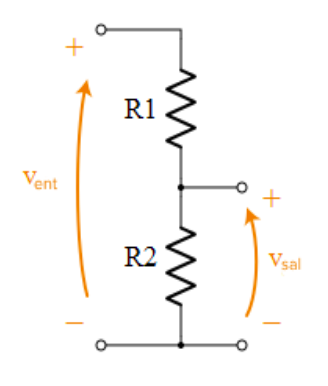
\includegraphics[width=55mm]{./Figuras/Nota_teorica/DTD}
\caption{Circuito de división de tensión.(Tomada de \cite{DT})}
\label{fig:DTD}
\end{figure}

Al pasar el diagrama anterior a expresiones matemáticas, de obtiene lo siguiente: 

\begin{equation}
    V_{sal} = V_{ent} \cdot \frac{R_{2}}{R_{1}+R_{2}} 
\end{equation}

Para el presente diseño, se seleccionó $R_{2} = 6.8 \; k\Omega$, además se sabe que la tensión de entrada es de 9 V y la tensión de salida debe ser de 5 V, por lo que sólo resta despejar el valor $R_1$: 

\begin{equation*}
    V_{sal} = V_{ent} \cdot \frac{R_{2}}{R_{1}+R_{2}} 
\end{equation*}

\begin{equation*}
    V_{sal} \cdot (R_{1}+R_{2}) = V_{ent} \cdot R_{2}
\end{equation*}

\begin{equation*}
    V_{sal} \cdot R_{1} + V_{sal} \cdot R_{2} = V_{ent} \cdot R_{2}
\end{equation*}

\begin{equation*}
    V_{sal} \cdot R_{1} = R_{2} \cdot (V_{ent} - V_{sal})
\end{equation*}

\begin{equation}
    R_{1} = R_{2} \cdot \frac{(V_{ent} - V_{sal})}{ V_{sal}}
\end{equation}

Sustituyendo los valores conocidos: 

\begin{equation}
    R_{1} = (6.8 \times 10^3) \cdot \frac{(9 - 5)}{5} = 5.44 \times 10^3 = 5.44 \; k\Omega
\end{equation}

Se selecciona un valor estándar, por lo que $R_1 = 5.6 \; k\Omega$. Lo anterior permitirá evitar sobrecargas de tensión en el microcontrolador y mantener su funcionamiento en condiciones controladas. 

\subsection{Lista de componentes y precios}

En la Tabla \ref{table:Equipo} pueden consultarse los componentes utilizados y sus precios, tomando como referencia los precios del sitio web de la tienda de componentes MicroJPM (\url{https://www.microjpm.com/}) y la página oficial de ST (\url{https://www.st.com/content/st_com/en.html}): 

\begin{table}[H]
\caption{Lista de componentes.}
\begin{center}
\begin{tabular}{c|c|c}
\hline
\textbf{Componente}&\textbf{Cantidad}&\textbf{Precio}\\
\hline
STM34F429I-DISC1 & 1 & \$29.30\\
Resistor de  k$\Omega$ & 1 & \$0,07\\
Resistor de  k$\Omega$ & 1 & \$0,07\\
Batería de 9 V $\Omega$ & 1 & \$5.64\\
\hline
Total & - & \$35.08\\
\end{tabular} \label{table:Equipo}
\end{center}
\end{table}

Según la Tabla \ref{table:Equipo}, para realizar este proyecto son necesario ₡18 073,50, según el valor del dólar al momento de escribir el presente informe. 